\RequirePackage{plautopatch}
\documentclass[14pt,aspectratio=169,xcolor=dvipsnames,table,onlytextwidth,dvipdfmx]{beamer}
\usepackage[utf8]{inputenc}
\usepackage{bxdpx-beamer} % dvipdfmxなので必要

\usetheme{Boadilla}
%Beamerフォント設定
\usefonttheme{professionalfonts}
\usepackage[T1]{fontenc}
\usepackage[deluxe,uplatex]{otf} % 日本語多ウェイト化
\usepackage{mlmodern}  % 太いComputer Modern
% MLmodernのバグを修正: cf. https://tex.stackexchange.com/questions/646333/size-of-integral-symbol-in-section-header-with-mlmodern
\DeclareFontFamily{OMX}{mlmex}{}
\DeclareFontShape{OMX}{mlmex}{m}{n}{%
   <->mlmex10%
   }{}
\usepackage{newtxtext} % 数式以外をTXフォントで上書き
% \usepackage[noalphabet,unicode]{pxchfon}
% \setminchofont{KozMinPro-Regular.otf}% 游明朝Regular
% \setboldminchofont{KozMinPro-Bold.otf}% 游明朝Demibold
% \setgothicfont[0]{BIZ-UDGothicR.ttc}% BIZ UDゴシックR
% \setboldgothicfont[0]{BIZ-UDGothicB.ttc}% BIZ UDゴシックB
\renewcommand{\familydefault}{\sfdefault}  % 英文をサンセリフ体に
\renewcommand{\kanjifamilydefault}{\gtdefault}  % 日本語をゴシック体に
\usefonttheme{structurebold} % タイトル部を太字
\setbeamerfont{alerted text}{series=\bfseries} % Alertを太字
\setbeamerfont{section in toc}{series=\mdseries} % 目次は太字にしない
\setbeamerfont{frametitle}{size=\Large} % フレームタイトル文字サイズ
\setbeamerfont{title}{size=\LARGE} % タイトル文字サイズ
\setbeamerfont{date}{size=\small}  % 日付文字サイズ
\usepackage{bxcoloremoji}

% Babel (日本語の場合のみ・英語の場合は不要)
\uselanguage{japanese}
\languagepath{japanese}
\deftranslation[to=japanese]{Theorem}{定理}
\deftranslation[to=japanese]{Lemma}{補題}
\deftranslation[to=japanese]{Example}{例}
\deftranslation[to=japanese]{Examples}{例}
\deftranslation[to=japanese]{Definition}{定義}
\deftranslation[to=japanese]{Definitions}{定義}
\deftranslation[to=japanese]{Problem}{問題}
\deftranslation[to=japanese]{Solution}{解}
\deftranslation[to=japanese]{Fact}{事実}
\deftranslation[to=japanese]{Proof}{証明}
\deftranslation[to=japanese]{Corollary}{系}
\setbeamertemplate{theorems}[normal font] %日本語の場合，定理内を斜体にしない
% overlay-aware proof environment
\renewenvironment<>{proof}{%
\par
\begin{actionenv}#1%
\structure{(証明)}}
{\qed\end{actionenv}}

%Beamer色設定
\definecolor{UniBlue}{RGB}{0,150,200}
\definecolor{UniGreen}{RGB}{3,175,122}
\definecolor{UniPink}{RGB}{255,128,255}
\definecolor{AlertOrange}{RGB}{255,76,0}
\definecolor{AlmostBlack}{RGB}{38,38,38}
\setbeamercolor{normal text}{fg=AlmostBlack}  % 本文カラー
\setbeamercolor{structure}{fg=UniBlue} % 見出しカラー
\setbeamercolor{block title}{fg=UniBlue!50!black} % ブロック部分タイトルカラー
\setbeamercolor{alerted text}{fg=AlertOrange} % \alert 文字カラー
\setbeamercolor{bibliography entry author}{fg=AlmostBlack} % Bib 文字カラー
\setbeamercolor{bibliography entry note}{fg=AlmostBlack} % Bib 文字カラー
\mode<beamer>{
    \definecolor{BackGroundGray}{RGB}{254,254,254}
    \setbeamercolor{background canvas}{bg=BackGroundGray} % スライドモードのみ背景をわずかにグレーにする
}

%フラットデザイン化
\setbeamertemplate{blocks}[rounded] % Blockの影を消す
\useinnertheme{circles} % 箇条書きをシンプルに
\setbeamertemplate{navigation symbols}{} % ナビゲーションシンボルを消す
\setbeamertemplate{footline}[frame number] % フッターはスライド番号のみ

%タイトルページ
\setbeamertemplate{title page}{%
    \vspace{2.5em}
    {\usebeamerfont{title} \usebeamercolor[fg]{title} \inserttitle \par}
    {\usebeamerfont{subtitle}\usebeamercolor[fg]{subtitle}\insertsubtitle \par}

    \vspace{1.5em}
    \begin{columns}[]
        \begin{column}{.35\linewidth}
        \usebeamerfont{titlegraphic}\inserttitlegraphic\par
        \end{column}
        \begin{column}{.6\linewidth}\setlength\topsep{0pt}
            \begin{flushright}
        \usebeamerfont{author}\insertauthor\par
        \usebeamerfont{institute}\insertinstitute \par
        \vspace{3em}
        \usebeamerfont{date}\insertdate\par
            \end{flushright}
        \end{column}
    \end{columns}
}

%biblatex
% \usepackage[style=ext-authoryear,citestyle=authoryear,natbib=true,giveninits=true,maxbibnames=99,maxcitenames=10,url=false,isbn=false,doi=false,articlein=false]{biblatex}
% \DeclareNameAlias{author}{first-last}
% \addbibresource{shrunk.bib}
% \newcommand{\mkbibbracketscol}[1]{\textcolor{UniBlue}{\scriptsize \mkbibbrackets{#1}}}
% \DeclareCiteCommand{\cite}[\mkbibbracketscol]
%   {\usebibmacro{prenote}}
%   {\usebibmacro{citeindex}%
%    \usebibmacro{cite}}
%   {\multicitedelim}
%   {\usebibmacro{postnote}}
% % \renewcommand{\cite}[1]{\textcolor{UniBlue}{\scriptsize\citep{#1}}}
% \renewcommand*{\finalnamedelim}{\addcomma\addspace} % remove "and" before the last author
% \DeclareDelimFormat{nameyeardelim}{\addspace}
% \setbeamertemplate{bibliography item}{}

% Algorithm系
\usepackage{algorithm}
\usepackage[noend]{algorithmic}
\algsetup{linenosize=\color{fg!50}\footnotesize}
\renewcommand\algorithmicdo{:}
\renewcommand\algorithmicthen{:}
\renewcommand\algorithmicrequire{\textbf{Input:}}
\renewcommand\algorithmicensure{\textbf{Output:}}
\renewcommand\algorithmiccomment[1]{\hfill\textcolor{fg!50}{\footnotesize\textit{// #1}}}

% TikZ
\usepackage{tikz}
\usetikzlibrary{positioning,shapes,arrows,quotes,shapes.callouts,calc,graphs,graphs.standard,fit,backgrounds,perspective,matrix}
\tikzset{point/.style={circle, fill=AlertOrange, inner sep=1pt, text width=1pt}}
\tikzset{bpoint/.style={circle, fill=black, inner sep=1pt, text width=1pt}}
\tikzset{alt/.code args={<#1>#2#3}{\alt<#1>{\pgfkeysalso{#2}}{\pgfkeysalso{#3}}}}
\tikzset{>=latex}
\tikzset{mynodes/.style={circle,white,fill=UniBlue!90,text width=.8em,inner sep=0pt,text centered,font=\footnotesize}}
\tikzset{myedges/.style={thick}}
\tikzset{mypath/.style={ultra thick, draw=#1}, mypath/.default=AlertOrange}
\tikzset{mysubset/.style={draw,#1,dotted,thick,fill=#1!10}, mysubset/.default=UniBlue}
\tikzset{mypath2/.style={ultra thick, dashed, draw=UniGreen}}
\tikzset{graphs/mygraph/.style={nodes={mynodes}, edges={myedges}, empty nodes}}
\tikzset{nomargin/.style={inner sep=0pt, outer sep=0pt}}
%% graph macros
\tikzgraphsset{declare={mybipartite}{%
subgraph I_nm [V={1,2,3,4,5,6}, W={a,b,c,d,e,f}];
1 -- {a,b};
2 -- {b,c,d,e};
3 -- {d,f};
4 -- {e,f};
{5,6} -- f;
}}
\tikzgraphsset{declare={mybipartitedi}{%
subgraph I_nm [V={1,2,3,4,5,6}, W={a,b,c,d,e,f}];
1 -> {a,b};
2 -> {b,c,d,e};
3 -> {d,f};
4 -> {e,f};
{5,6} -> f;
}}
\tikzgraphsset{declare={mybipartite2}{%
subgraph I_nm [V={1,2,3}, W={a,b,c}];
1 -- {a,b}; 2 -- {a,b,c}; 3 -- {a,c};
}} 
% Petersen graph
\tikzgraphsset{declare={Petersen}{%
    subgraph C_n [n=5,name=A, radius=1.5cm]; 
    subgraph I_n [n=5,name=B, radius=.8cm];
    \foreach \i [evaluate={\j=int(mod(\i+2,5)+1);}] in {1,...,5}{
        A \i -- B \i;
        B \i -- B \j;
}}}
% Example graph for Menger's theorem
\tikzgraphsset{declare={menger}{%
    s[at={(-1,0)}, as={$s$}];
    (s) -> 1[at={(0,1)}] -> 2[at={(1,0)}];
    (s) -> 3[at={(0,-1)}] -> 2;
    4[at={(2,1)}] <- 5[at={(2,-1)}];
    {5,6[at={(3,1)}], 7[at={(3,-1)}]} -> t[at={(4,0)}, as={$t$}];
    (s) -> (2);
    (2) -> {(4), (5)};
    {(4),(5)} -> {(6),(7)};
    (6) -> (7);
    1 -> 4;
}} 
\tikzgraphsset{declare={undirected menger}{%
    s[at={(-1,0)}, as={$s$}];
    (s) -- 1[at={(0,1)}] -- 2[at={(1,0)}];
    (s) -- 3[at={(0,-1)}] -- 2;
    4[at={(2,1)}] -- 5[at={(2,-1)}];
    {5,6[at={(3,1)}], 7[at={(3,-1)}]} -- t[at={(4,0)}, as={$t$}];
    (s) -- (2);
    (2) -- {(4), (5)};
    {(4),(5)} -- {(6),(7)};
    (6) -- (7);
    1 -- 4;
}} 

% Appendix
\usepackage{appendixnumberbeamer}

% macros
\newcommand{\R}{\mathbb{R}}
\newcommand{\Z}{\mathbb{Z}}
\newcommand{\be}{\mathbf{e}}
\newcommand{\zeros}{\mathbf{0}}
\newcommand{\ones}{\mathbf{1}}
\newcommand{\bfzero}{\zeros}
\newcommand{\bfone}{\ones}

% \newcommand{\bp}{\mathbf{p}}
\newcommand{\eps}{\varepsilon}
\newcommand{\defiff}{\overset{\text{def}}{\iff}}
\DeclareMathOperator{\poly}{poly}
\DeclareMathOperator{\conv}{conv}
\DeclareMathOperator{\In}{In}
\DeclareMathOperator{\Out}{Out}
\DeclareMathOperator{\val}{val}
\newcommand{\lo}{{\mathrm{lo}}}
\newcommand{\up}{{\mathrm{up}}}
\newcommand{\caI}{\mathcal{I}}
\newcommand{\caB}{\mathcal{B}}
\newcommand{\caC}{\mathcal{C}}
\newcommand{\bM}{\mathbf{M}}
\newcommand{\IO}{\mathrm{IO}}

\usepackage{mathtools}
\DeclarePairedDelimiter{\abs}{\lvert}{\rvert}
\DeclarePairedDelimiter{\norm}{\lVert}{\rVert}
\DeclarePairedDelimiter{\inprod}{\langle}{\rangle}
\usepackage[no-test-for-array]{nicematrix}
\usepackage{diagbox}

\newcommand{\highlightcap}[3][red]{\tikz[baseline=(x.base)]{\node[rectangle,rounded corners,fill=#1!10](x){#2} node[below=0pt of x, color=#1]{#3};}}
\newcommand{\highlight}[2][red]{\tikz[baseline=(x.base)]{\node[rectangle,rounded corners,fill=#1!10](x){#2};}}
\newcommand{\mycite}[2][\footnotesize]{\textcolor{UniBlue}{#1 [#2]}}

%section
% \AtBeginSection[]{
%     \frame[c]{
%         \centering
%         \begin{tikzpicture}
%             \node[white, circle, fill=UniBlue, text centered, text width=.3\linewidth](bullet) {
%                 {\Huge \bf \insertsectionnumber} \\[4em]
%     };
%     \node[text width=.65\linewidth, right=1em of bullet]{%
%         \usebeamerfont{title}\usebeamercolor[fg]{title}\insertsection\par %
%     };
%         \end{tikzpicture}
%     } %目次スライド
% }

%grid
% \usepackage[colorgrid,gridunit=pt,texcoord]{eso-pic}
\newcommand{\postit}[1]{\tikz[overlay, remember picture]{\node[draw,anchor=north east, align=center, rectangle, fill=yellow!10, xshift=-1pt, yshift=-1pt] at (current page.north east) {#1};}}

\usepackage{tcolorbox}
\newtcolorbox{primal}{colback=red!10!white, colframe=red, title=主問題 (P), left=2pt,right=2pt,top=0pt,bottom=0pt}
\newtcolorbox{dual}{colback=blue!10!white, colframe=blue, title=双対問題 (D), left=2pt,right=2pt,top=0pt,bottom=0pt}

% visible on
\usetikzlibrary{overlay-beamer-styles}
\usepackage[normalem]{ulem}
\usepackage{pxrubrica}
\usepackage{booktabs}

\newcommand{\Aphiup}{\textcolor{UniBlue}{A_\varphi^\up}}
\newcommand{\Aphilow}{\textcolor{AlertOrange}{A_\varphi^\lo}}
\newcommand{\bv}{\boldsymbol{v}}
\newcommand{\bx}{\boldsymbol{x}}
\newcommand{\by}{\boldsymbol{y}}
\newcommand{\bz}{\boldsymbol{z}}
\newcommand{\bw}{\boldsymbol{w}}
\newcommand{\bc}{{\boldsymbol c}}
\DeclareMathOperator{\supp}{supp}
\DeclareMathOperator{\argmax}{argmax}
\DeclareMathOperator{\argmin}{argmin}
\DeclareMathOperator{\E}{\mathbb{E}}
\csname endofdump\endcsname
\title{組合せ最適化特論}
\subtitle{第4回（最大流①）}
\author{担当: \textbf{相馬 輔}}
\date{2026/5/21}

\begin{document}
\maketitle

\begin{frame}{}
    \centering\small
    \tikzset{block/.style={rectangle, draw=gray, fill=gray!10, thick, minimum width=3em, minimum height=2em, align=center}}
    \begin{tikzpicture}
        \node[block,] (BM) {重みなし\\二部マッチング};
        \node[block,above=1em of BM.north west, xshift=-2em] (WBM) {重みつき\\二部マッチング};
        \node[block,above=5em of BM.north east, xshift=1em] (NF) {最大流};
        \node[block,above=9em of BM] (MCF) {最小費用流};
        % \node[block,above=1em of NF.north east, xshift=1em] (MC) {最小カット};
        \node[block,right=11em of BM] (MTR) {マトロイド};
        \node[block,above=7em of MTR] (MI) {マトロイド交差};
        \node[block,above=3em of MCF, xshift=7em] (SFM) {劣モジュラ最小化};
        \graph[mygraph]{
            (BM) -> {(WBM), (NF)} -> (MCF);
            {(MTR), (BM)} -> (MI);
            % (NF) -> (MC);
            {(MCF), (MI)} -> (SFM);
        };
        \begin{scope}[on background layer]
            \node[mysubset, fit=(BM) (WBM), "二部マッチング" {below, UniBlue}]{};
            \node[mysubset, AlertOrange, fill=AlertOrange!10, fit=(NF) (MCF), "ネットワークフロー" {above left, AlertOrange}]{};
            \node[mysubset, UniGreen, fill=UniGreen!10, fit=(MTR) (MI), "マトロイド" {below, UniGreen}]{};
        \end{scope}
    \end{tikzpicture}
\end{frame}

\begin{frame}[allowframebreaks]
    \frametitle{各回の内容（予定）} 
    \small
    \begin{enumerate}
        \item (4/23) イントロ+多面体的組合せ論（線形計画法の復習，整数多面体，完全単模行列）
        \item[] \textcolor{gray}{(4/30) 休み}
        \item (5/7) 二部マッチング①（Konig-Egervaryの定理，増加道アルゴリズム，ハンガリー法）
        \item (5/14) 二部マッチング②（最短路問題の復習，逐次最短路法と主双対法，最適性基準からの見方）
        \item (5/21) 最大流① （定式化，最大流最小カット定理，応用例）
        \item (5/28) 最大流②（残余ネットワーク，Ford--Fulkerson法，Edmonds--Karpのアルゴリズム）+ 最小費用流①（定式化，輸送問題，最大流との関係）
        \item[] \textcolor{gray}{(6/4) 休み}
        % \item[] \sout{(12/11) 最小カット（永持茨木のアルゴリズム，Kargerのアルゴリズム）}
        \item (6/11) 最小費用流②（逐次最短路法，容量スケーリング法）
        \item[] \textcolor{gray}{(6/18) 休み}
        \item[] \textcolor{gray}{(6/25) 休み}
        \item (7/2) マトロイド（定義と公理系，貪欲法，マトロイド多面体） 
        \item (7/9) 独立マッチング・マトロイド交差 （定義，応用例，Edmondsの最大最小定理，増加道アルゴリズム）
        \item (7/16) 劣モジュラ関数①（諸例，劣モジュラ基多面体，Lov\'asz拡張，劣モジュラ最小化）
        \item[] \textcolor{gray}{(7/23) 休み}
        \item (7/30) 劣モジュラ関数②（劣モジュラ最大化，近似アルゴリズム，貪欲法）
        \item (どこか) 精選トピック①
        \item (どこか) 精選トピック②
        \item (どこか) 精選トピック③
    \end{enumerate}

    \bigskip
    \begin{itemize}
        \item レポート課題を6月と期末に出す予定
        \item 精選トピックの日時は今後調整 
    \end{itemize}
\end{frame}

\begin{frame}<1>[label=outline]{目次}
\begin{tikzpicture}
    \tikzstyle{block} = [rectangle, text width=\textwidth, rounded corners, minimum height=4em]
    \tikzstyle{line} = [draw, -latex]

    \node[block,alt={<1,3->{fill=cyan!10}{fill=red!10}}] (combopt) {
        \begin{columns}
            \begin{column}{0.5\linewidth}
        \textbf{1. 最大流問題}
            \end{column}
            \begin{column}{0.4\linewidth}
                \small
                \structure{・} 定義\\
                \structure{・} 最大流最小カット定理 \\
                \structure{・} 整数性 \\
            \end{column}
        \end{columns}
    };
    \node[block,alt={<1-2,4->{fill=cyan!10}{fill=red!10}}, below=.5em of combopt] (LP) {
        \begin{columns}
            \begin{column}{0.5\linewidth}
        \textbf{2. 最大流を用いたモデリング}
            \end{column}
            \begin{column}{0.4\linewidth}
                \small
                \structure{・} Mengerの定理 \\
                \structure{・} 二部マッチング \\
                \structure{・} Baseball Elimination \\
                \structure{・} 最密部分グラフ
            \end{column}
        \end{columns}
    };
\end{tikzpicture}%

\bigskip
\hfill ※アルゴリズムは次回
\end{frame}

%%%%%%%%%%%%%%%%%%%%%%%%%%%%%%%%%%%%%%%%%%%%%
\section{最大流問題}
\againframe<2|handout:0>{outline}
%%%%%%%%%%%%%%%%%%%%%%%%%%%%%%%%%%%%%%%%%%%%%

\begin{frame}{\insertsection :定義}
    $G = (V, A)$: 有向グラフ 

    \begin{definition}
        $\varphi: A \to \R$に対し，その\alert{境界} $\partial \varphi: V \to \R$を
        \[
            (\partial\varphi)(i) := \sum_{a \in \Out(i)} \varphi(a) - \sum_{a \in \In(i)} \varphi(a)  \qquad (i \in V)
        \]
        と定義する．ここで，$\In(i)$, $\Out(i)$はそれぞれ頂点$i$に入る枝，出る枝の集合．

        {\hfill\footnotesize ※$\delta^+(i)$, $\delta^-(i)$と表記する本もある．}
    \end{definition}
\end{frame}

\begin{frame}{\insertsection :定義}
    $G = (V, A)$: 有向グラフ, $u: A \to \R_+$: 枝容量関数 \\
    $s, t \in V$: 始点, 終点 

    \begin{definition}[$s$--$t$流]
        $\varphi: A \to \R$が\alert{$s$--$t$\ruby{流}{フロー}} $\defiff$
        \begin{itemize}
            \item $0 \leq \varphi(a) \leq u(a)$ \qquad ($a \in A$) \hfill \textbf{（容量制約）} 
            \item $(\partial\varphi)(i) = 0$ \qquad ($i \in V \setminus \{s, t\}$) \hfill \textbf{（流量保存則）}
        \end{itemize}
    \end{definition}

    \pause
    \begin{block}{最大流問題 (Maximum Flow Problem)}
        $s$--$t$流$\varphi$で\alert{流量} \[
            \val(\varphi) := (\partial\varphi)(s) = -(\partial\varphi)(t) 
        \]
        が最大のものを求めよ．
    \end{block}
\end{frame}

\begin{frame}[label=flow-example]{例}
    \textcolor{UniBlue}{$\varphi$}: 流量 / $u$: 容量

    \begin{center}
    \begin{tikzpicture}[scale=1.6]

        \graph[no placement, mygraph]{
            s[at={(0,0)}, as={$s$}];
            a[at={(2, 1)}];
            b[at={(2,-1)}];
            c[at={(4, 1)}];
            d[at={(4,-1)}];
            t[at={(6, 0)}, as={$t$}];
        };
        \foreach \i/\j/\f/\u in {
            s/a/5/5,
            s/b/2/3,
            a/b/1/2,
            a/c/3/3,
            a/d/1/2,
            b/d/3/4,
            c/t/4/5,
            d/c/1/1,
            d/t/3/3
        } {
            \path[myedges,->] (\i) edge node[above, midway, sloped] {\small \textcolor{UniBlue}{$\f$} / $\u$} (\j);
        }
    \end{tikzpicture}
    \end{center}

    流量: $7$ （実は最大流）
\end{frame}

\begin{frame}{\insertsection :線形計画問題として}
    \footnotesize
    \begin{primal}
        \setlength{\abovedisplayskip}{0pt}
        \begin{alignat*}{3}
            \text{max}   \quad & \sum_{a \in \Out(s)} \varphi(a) && \quad \\
            \text{s.t.}  \quad & \sum_{a \in \Out(i)} \varphi(a)  - \sum_{a \in \In(i)} \varphi(a) = 0 && \quad (i \in V \setminus \{s, t\}) \\
                         \quad & 0 \leq \varphi(a) \leq u(a) && \quad (a \in A)
        \end{alignat*}
    \end{primal}
    \begin{dual}
        \setlength{\abovedisplayskip}{0pt}
        \only<1>{
        \begin{alignat*}{3}
            \text{min}  \quad & \sum_{a \in A} u(a) y(a)   && \\
            \text{s.t.} \quad & x(j) \phantom{{}-{}x(i)} + y(a) &&\;\geq 1  \quad && (a=sj \in \Out(s)) \\
                        \quad & \phantom{x(i) } -x(i) + y(a)    &&\;\geq 0  \quad && (a=it \in \In(t)) \\
                        \quad & x(j) - x(i) + y(a)              &&\;\geq 0  \quad && (a=ij \in A \setminus \Out(s) \cup \In(t)) \\
                        \quad & y(a)                            &&\;\geq 0  \quad && (a \in A)
        \end{alignat*}
        }
        \only<2>{
        \begin{alignat*}{3}
            \min_{x \in \R^V} & \quad \sum_{a=ij \in A} u(a) \max\{x(i) - x(j), 0\}   \\
            \text{s.t.} &\quad  x(s) = 1  \\
                        &\quad  x(t) = 0 
        \end{alignat*}
        }
    \end{dual}
\end{frame}

\begin{frame}{\insertsection :整数性}
    \small
    \begin{columns}
    \begin{column}{.7\textwidth}
    \structure{ネットワーク行列} 有向グラフ$G = (V, A)$に対し，\\ 
    $V \times A$行列$B$を
    \[
        B_{i,a} := \begin{cases}
            +1 & \text{($i$は$a$の始点)} \\
            -1 & \text{($i$は$a$の終点)} \\
            0  & \text{otherwise}
        \end{cases} 
    \]
    $(i \in V, a \in A)$と定める．
    \end{column}
    \begin{column}{.3\textwidth}
        \centering
        \begin{tikzpicture}
            \graph[mygraph, math nodes]{
            a -> b;
            c -> d;
            a -> d;
        };
        \end{tikzpicture}
        \[
            B = \begin{bmatrix}
                +1 & +1 & 0 \\
                -1 & 0 & 0 \\
                0 & 0 & +1 \\
                0 & -1 & -1 \\
            \end{bmatrix}
        \]
    \end{column}
    \end{columns}

    \bigskip
    \begin{lemma}
        ネットワーク行列は\alert{完全単模行列}．
    \end{lemma}
\end{frame}

\begin{frame}{\insertsection :整数性}
    最大流問題の係数行列は$
        \begin{bmatrix}
            \tilde B \\
            I
        \end{bmatrix}$. ここで$\tilde B$は$B$から$s$と$t$の行を除いたもの．
    ネットワーク行列の完全単模性より，この行列も完全単模．

    \vfill
    完全単模行列とLPの整数性（第1回参照）から，以下の定理が従う．

    \begin{theorem}
        最大流問題には整数双対最適解が存在する．
        さらに，枝容量$u$が整数値のときは，整数値の最大流が存在する．
    \end{theorem}

\end{frame}

\begin{frame}{最大流最小カット定理}
    \small
    \begin{columns}[T]
    \begin{column}{.7\textwidth}
    \begin{definition}
        \begin{itemize}
            \item $X \subseteq V$が\alert{$s$--$t$カット} $\defiff s \in X, t \not\in X$
            \item $s$--$t$カット$X$の\alert{容量}: $u(\Out(X)) = \sum_{a \in \Out(X)} u(a)$
        \end{itemize}
    \end{definition}
    \end{column}
    \begin{column}{.3\textwidth}
    \centering

    \begin{tikzpicture}[scale=0.6]
        \graph[no placement, mygraph]{
            s[at={(0,0)}, as={$s$}];
            a[at={(2, 1)}];
            b[at={(2,-1)}];
            c[at={(4, 1)}];
            d[at={(4,-1)}];
            t[at={(6, 0)}, as={$t$}];
            s -> {a, b} -> {c, d} -> t;
            a -> {b, d};
            c -> d;
            {[edges={mypath}]
                a -> {c, d};
                b -> d;
            }
        };
        \node[AlertOrange, above] at ($(a)!.5!(c)$) {$\Out(X)$};
        \begin{scope}[on background layer]
        \node[mysubset, fit=(s) (a) (b),"{$X$}" {below, UniBlue}] {};
        \end{scope}
    \end{tikzpicture}
        % \tikz{\graph[mygraph, no placement]{
        %     subgraph C_n [n=4, clockwise];
        %     5[at={(3,0)}] -- 6[at={(2,1)}] -- 7[at={(2,-1)}] -- ;
        %     {[edges={mypath}]
        %         {(1),(2)} -- (6);
        %         {(2),(3)} -- (7);
        %     };
        % };
    \end{column}
    \end{columns}

    \pause
    \bigskip
    \structure{弱双対性} 任意の$s$--$t$流$\varphi$と$s$--$t$カット$X$に対し，次が成り立つ．
    \[
        \val(\varphi) \leq u(\Out(X))
    \]

    \pause
    \bigskip
    \begin{alertblock}{最大流最小カット定理 (Ford--Fulkerson, 1956; Danzig--Fulkerson, 1956)}
        \[
            \max_{\text{$\varphi$:~$s$--$t$流}} \val(\varphi) = \min_{\text{$X$:~$s$--$t$カット}} u(\Out(X)) 
        \]
    \end{alertblock}
    次回，アルゴリズム的な証明を与える．
\end{frame}

\againframe{flow-example}

\begin{frame}{実例: 冷戦時代}
    \centering
    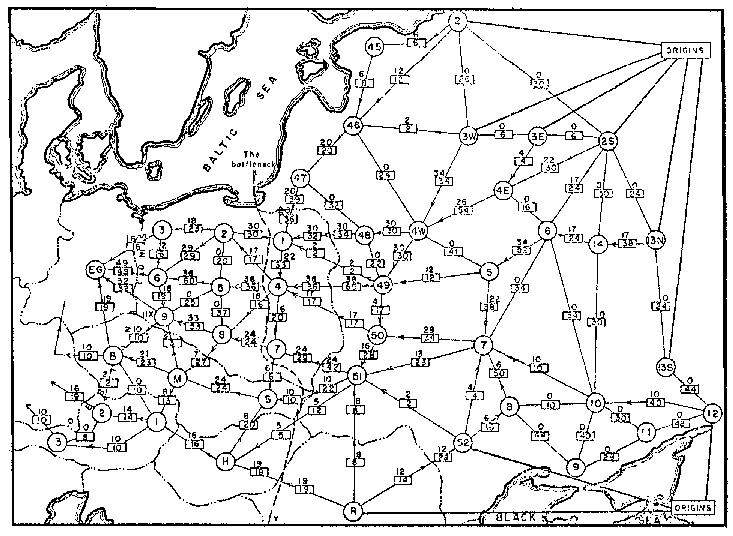
\includegraphics[height=0.8\textheight]{figs/coldwar_cropped.pdf} \\ 
    \scriptsize 出典 Harris, T.E., Ross, F.S. (1955): Fundamentals of a Method for Evaluating Rail Net Capacities. Research Memorandum RM-1573, The RAND Corporation, Santa Monica, California
\end{frame}

%%%%%%%%%%%%%%%%%%%%%%%%%%%%%%%%%%%%%%%%%%%%%
\section{最大流を用いたモデリング}
\againframe<3|handout:0>{outline}
%%%%%%%%%%%%%%%%%%%%%%%%%%%%%%%%%%%%%%%%%%%%%

\begin{frame}<1-2>[label=modeling]{\insertsection}
    最大流を用いたモデリングの例として以下を紹介する: 

    \bigskip
    \begin{enumerate}[<alert@+(1)>]
        \setlength{\itemsep}{1em}
        \item Mengerの定理 (点素・辺素パス問題)
        \item 二部マッチング
        \item Baseball Elimination
        \item 最密部分グラフ問題 (密グラフ抽出)
    \end{enumerate}
\end{frame}


\subsection{Mengerの定理}
\begin{frame}
    \frametitle{辺素・点素パス問題}

    \begin{columns}[T]
    \begin{column}{.6\textwidth}
    \begin{block}{有向$s$--$t$辺素パス問題}
        \structure{入力:} 有向グラフ $G = (V, A)$, $s, t \in V$  \\
        \structure{出力:} 辺素$s$--$t$パスの最大集合
    \end{block}
    \end{column}
    \begin{column}{.4\textwidth}
        \centering
        \tikz{\graph[mygraph,no placement]{
            menger;
            % edge-disjoint paths
            {[edges={mypath}]
                (s) -> (1) -> (2) -> (4) -> (6) -> (t); 
                (s) -> (3) -> (2) -> (5) -> (7) -> (t);
            }
        };} \\
        辺素$s$--$t$パス
    \end{column}
    \end{columns}

    \vfill\pause
    \begin{columns}[T]
    \begin{column}{.6\textwidth}
    \begin{block}{有向$s$--$t$点素パス問題}
        \structure{入力:} 有向グラフ $G = (V, A)$, $s, t \in V$  \\
        \structure{出力:} 点素$s$--$t$パスの最大集合
    \end{block}
    \end{column}
    \begin{column}{.4\textwidth}
        \centering
        \tikz{\graph[mygraph,no placement]{
            menger;
            % vertex-disjoint paths
            {[edges={mypath}]
                s -> 1 -> 4 -> 6 -> t; 
                s -> 3 -> 2 -> 5 -> 7 -> t;
            }
        };} \\
        点素$s$--$t$パス
    \end{column}
    \end{columns}
\end{frame}

% \begin{frame}
%     \frametitle{Cuts}

%     \begin{columns}[T]
%     \begin{column}{.7\textwidth}
%         \begin{itemize}
%             \item 
%     For a vertex subset $X \subseteq V$, let the \alert{cut} of $X$ be
%     \[
%         E[X, \bar X] = \{uv \in E : u \in X, v \not\in X\}.
%     \]
%             \item For $s, t \in V$, an \alert{$s$--$t$ cut} is a cut for $X$ s.t. $s \in X$ and $t \notin X$.
%         \end{itemize}
%     \end{column}
%     \begin{column}{.3\textwidth}
%     \centering
%         \tikz{\graph[mygraph, no placement]{
%             subgraph C_n [n=4, clockwise];
%             5[at={(3,0)}] -- 6[at={(2,1)}] -- 7[at={(2,-1)}] -- (5);
%             {[edges={mypath}]
%                 {(1),(2)} -- (6);
%                 {(2),(3)} -- (7);
%             };
%         };
%         \node[AlertOrange, above] at ($(1)!.5!(6)$) {$E[X, \bar X]$};
%         \begin{scope}[on background layer]
%         \node[mysubset, fit=(1) (2) (3) (4),"{$X$}" {below, UniBlue}] {};
%         \end{scope}
%         }
%     \end{column}
%     \end{columns}

%     \vfill\pause
%     \structure{Observation} \\
%     % $G$ is $k$-edge connected $\implies$ $\abs{E[X, \bar X]} \geq k$ for $\emptyset \neq \forall X \subsetneq V$.
%     Maximum number of edge disjoint $s$--$t$ paths $\leq$ minimum size of $s$--$t$ cut.
%     \begin{center}
%     \bf It's actually tight! (Menger's theorem)
%     \end{center}
% \end{frame}

\begin{frame}
    \frametitle{Mengerの定理（有向・辺素ver）}
    \begin{columns}[T]
    \begin{column}{.6\textwidth}
    \begin{block}{Mengerの定理（有向・辺素ver）}
        辺素$s$--$t$パスの最大本数 \\
        $= \min\{ |\Out(X)| : \text{$s \in X \subseteq V \setminus t$}\}$
    \end{block}

    辺素$s$--$t$パスの本数$\leq |\Out(X)|$は自明．
    \end{column}
    \begin{column}{.4\textwidth}
    \centering
        \tikz{\graph[mygraph,no placement]{
            menger;
            % edge-disjoint paths
            {[edges={mypath}]
                (s) -> (1) -> (2) -> (4) -> (6) -> (t); 
                (s) -> (3) -> (2) -> (5) -> (7) -> (t);
            }
        };
            % min cut
            \begin{scope}[on background layer]
            % \node[mysubset, fit=(s) (1) (2) (3), "min $s$--$t$ cut (size $=2$)" {below, UniBlue}] {};
            \draw[mysubset] (s.west |- 1.north) -- ($(4.north east)!.5!(6.north west)$) -- (2.center |- 3.south) -- (3.south -| s.west) -- cycle;
            \node[below=1pt of 3, UniBlue, align=center] {最小$s$--$t$カット \\ ($|\Out(X)|=2$)};
            \end{scope}
        }
    \end{column}
    \end{columns}

    \vfill
    \pause
    \begin{proof}
    枝容量$u \equiv 1$として$s$--$t$最大流を考える．整数の$s$--$t$流は辺素$s$--$t$パスに対応する．また，最大流問題の整数性より，整数の$s$--$t$最大流が存在する．よって，Mengerの定理は最大流最小カット定理に他ならない． 
    \end{proof}
    % \structure{Connection to edge-connectivity}
    % \begin{corollary}
    %     $G$ is $k$-edge-connected \\
    %     $\iff$ $\abs{E[X, \bar X]} \geq k$ for $\emptyset \neq \forall X \subsetneq V$ \\
    %     $\iff$ $G$ has at least $k$ edge-disjoint $s$--$t$ paths for any distinct $s, t \in V$  
    % \end{corollary}
\end{frame}

\begin{frame}
    \frametitle{Mengerの定理（有向・点素ver）}

    \begin{columns}[T]
    \begin{column}{.6\textwidth}
    \begin{block}{Mengerの定理（有向・点素ver）}
        点素$s$--$t$パスの最大本数 \\
        $= \min\{ |U| : U \subseteq V \text{は$s$と$t$を分離} \}$
    \end{block}

    点素$s$--$t$パスの本数$\leq |U|$は自明．
    \end{column}
    \begin{column}{.4\textwidth}
    \centering
        \tikz{\graph[mygraph,no placement]{
            menger;
            % vertex-disjoint paths
            {[edges={mypath}]
                s -> 1 -> 4 -> 6 -> t; 
                s -> 3 -> 2 -> 5 -> 7 -> t;
            }
        };
            % min cut
        \begin{scope}[on background layer]
            \node[mysubset, fit=(4) (5), "最小$s$--$t$分離集合 ($|U|=2$)" {below, UniBlue}] {};
        \end{scope}
        }
    \end{column}
    \end{columns}

    \vfill
    \pause
    \begin{proof}
    $s,t$以外の各頂点を以下のように変換したネットワークで，最大流最小カット定理を適用すればよい．
    \begin{center}
        \tikz[baseline=(v.base)]{
        \graph[empty nodes, grow right=5em, branch down=1.5em]{
            subgraph I_nm[V={1,2,3}, W={a,b}];
        };
        \node[mynodes](v) at ($(2)!.5!(b)$) {$v$};
        \graph[mygraph]
        {
            {(1), (2), (3)} -> (v) -> {(a), (b)};
        };
        }
        \qquad $\longrightarrow$ \qquad
        \tikz[baseline=(v1.base)]{
        \graph[empty nodes, grow right=9em, branch down=1.5em]{
            subgraph I_nm[V={1,2,3}, W={a,b}];
        };
        \node[mynodes](v1) at ($(2)!.33!(b)$) {$v_1$};
        \node[mynodes](v2) at ($(2)!.66!(b)$) {$v_2$};
        \graph[mygraph]
        {
            {(1), (2), (3)} -> (v1) ->[UniGreen] (v2) -> {(a), (b)};
        };
        \path (v1) -- (v2) node[midway, above, sloped]{\footnotesize $1$};
        \path (1) -- (v1) node[midway, above, sloped]{\footnotesize $+\infty$};
        \path (v2) -- (a) node[midway, above, sloped]{\footnotesize $+\infty$};
        }
    \end{center}
    \end{proof}
\end{frame}

\begin{frame}{Mengerの定理（無向・点素ver）}
    Mengerの定理には無向グラフ版もある．
    
    \begin{columns}[T]
    \begin{column}{.6\textwidth}
    \begin{block}{無向$s$--$t$点素パス問題}
        \structure{入力:} 無向グラフ $G = (V, E)$, $s, t \in V$  \\
        \structure{出力:} 点素$s$--$t$パスの最大集合
    \end{block}
    \end{column}
    \begin{column}{.4\textwidth}
        \centering
        \tikz{\graph[mygraph,no placement]{
            undirected menger;
            % vertex-disjoint paths
            {[edges={mypath}]
                s -- 1 -- 4 -- 6 -- t; 
                s -- 3 -- 2 -- 5 -- 7 -- t;
            }
        };
        % min cut
        \begin{scope}[on background layer]
            \node[mysubset, fit=(4) (5), "最小$s$--$t$分離集合 ($|U|=2$)" {below, UniBlue}] {};
        \end{scope}
        } 
    \end{column}
    \end{columns}

    \bigskip
    \begin{block}{Mengerの定理（無向・点素ver）}
        点素$s$--$t$パスの最大本数
        $= \min\{ |U| : U \subseteq V \text{は$s$と$t$を分離} \}$
    \end{block}
    \begin{proof}
     各枝を両方向に向きづけた有向グラフに対し，有向・点素Mengerを使う． 
    \end{proof}
\end{frame}

\begin{frame}{Mengerの定理（無向・辺素ver）}
    
    \begin{columns}[T]
    \begin{column}{.6\textwidth}
    \begin{block}{Mengerの定理（無向・辺素ver）}
        辺素$s$--$t$パスの最大本数 \\
        $= \min\{ |E[X, \bar X]| : \text{$s \in X \subseteq V \setminus t$}\}$
    \end{block}
    \end{column}
    \begin{column}{.4\textwidth}
    \centering
        \tikz{\graph[mygraph,no placement]{
            undirected menger;
            % edge-disjoint paths
            {[edges={mypath}]
                (s) -- (1) -- (4) -- (6) -- (t); 
                (s) -- (2) -- (4) -- (5) -- (t);
                (s) -- (3) -- (2) -- (5) -- (7) -- (t);
            }
        };
            % min cut
            \begin{scope}[on background layer]
            \node[mysubset, fit=(s) (1) (2) (3), "\footnotesize 最小$s$--$t$カット (size $=3$)" {below, UniBlue}] {};
            % \draw[mysubset] (s.west |- 1.north) -- ($(4.north east)!.5!(6.north west)$) -- (2.center |- 3.south) -- (3.south -| s.west) -- cycle;
            % \node[below=1pt of 3, UniBlue, align=center] {最小$s$--$t$カット \\ ($|\Out(X)|=2$)};
            \end{scope}
        }
    \end{column}
    \end{columns}

    \begin{proof}
        各枝を以下のように変換した有向グラフで，有向・辺素Mengerを適用すればよい．
        \begin{center}
            \tikz[baseline=(i.base)]{
            \graph[mygraph, math nodes, grow right=5em, branch down=1.5em]{ i -- j };}
            \qquad $\longrightarrow$ \qquad
            \tikz[baseline=(i.base)]{
            \graph[mygraph, math nodes, no placement]{
                subgraph I_n[V={1,j,2,i}, clockwise];
                i -> 1 -> 2 -> j;
                j -> 1 -> 2 -> i;
            };
            }
        \end{center}
    \end{proof}
\end{frame}

\subsection{二部マッチング}
\againframe<3>{modeling}

\begin{frame}
    \frametitle{K\H{o}nig--Egerv\'aryの定理（復習）}
    \small

    $G = (V^+, V^-; E)$を$V^+, V^-$を頂点集合とする二部グラフとする．

    \begin{columns}[T]
    \begin{column}{.7\textwidth}
    \begin{definition}
        $S \subseteq V^+, T \subseteq V^-$ が\alert{頂点被覆} \\
        $\defiff$ 任意の枝$e = ij \in E$に対し，$i \in S$または$j \in T$.
    \end{definition}
    \bigskip
    \begin{theorem}[K\H{o}nig--Egerv\'ary]
        二部グラフ$G$において，次の最大最小定理が成り立つ．
        \[
            \max_{\text{$M$:マッチング}} |M| = \min_{\text{$(S,T)$: 頂点被覆}} |S| + |T|
        \]
    \end{theorem}
    \end{column}
    \begin{column}{.3\textwidth}
        \centering
        \tikz{
            \graph[mygraph, grow right=5em]{ mybipartite; };
            \graph[edges={mypath}] {{(1),(2),(3),(4),(5)} -- {(b),(c),(d),(e),(f)}; };
        \begin{scope}[on background layer]
            \node[mysubset, fit=(1) (2), "$S$" left ]{} ;
            \node[mysubset, fit=(d) (e) (f), "$T$" right]{} ;
        \end{scope}
        }
    \end{column}
    \end{columns}

\end{frame}

\begin{frame}{最大流最小カット $\implies$ K\H{o}nig--Egerv\'ary}
        \centering
        \tikz{
        \onslide<1>{
            \graph[mygraph,grow right=4em]{
            subgraph I_nm [V={1,2,3,4,5,6}, W={a,b,c,d,e,f}];
            1 -- {a,b};
            2 -- {b,c,d,e};
            3 -- {d,f};
            4 -- {e,f};
            {5,6} -- f;
        };
        }
        \onslide<2->{
            \graph[mygraph,grow right=4em]{
            subgraph I_nm [V={1,2,3,4,5,6}, W={a,b,c,d,e,f}];
            1 -> {a,b};
            2 -> {b,c,d,e};
            3 -> {d,f};
            4 -> {e,f};
            {5,6} -> f;
        };
        }
        \onslide<3->{
        \node[mynodes](s) at (-2,-2.5) {$s$};
        \node[mynodes](t) at ( 4,-2.5) {$t$};
        \node[above] at ($(1)!.5!(a)$) {\footnotesize $+\infty$};
        \node[below] at ($(6)!.5!(f)$) {\footnotesize $+\infty$};
        \graph[mygraph]{
            (s) -> {(1), (2), (3), (4), (5), (6)};
            (t) <- {(a), (b), (c), (d), (e), (f)};
        };
        \foreach \i\j in {s/1, s/2, s/6, a/t, b/t, f/t}{
            \path (\i) -- (\j) node[midway, above]{\footnotesize $1$};
        }
        }
        \onslide<4->{
        \graph[edges={mypath}]{
            (s) -> {(1), (2), (3), (4), (5)} -> {(b), (c), (d), (e), (f)} -> (t);
        };
        }
        % \begin{scope}[on background layer]
        % \onslide<5->{
        %     \node[mysubset, fit=(3) (4) (5) (6), "{$X$}" {below left, UniBlue}]{} ;
        %     \node[mysubset, fit=(d) (e) (f), "{$\Gamma(X)$}" {below right, UniBlue}]{} ;
        % }
        % \end{scope}
        }

    \begin{center}
        \small
    \onslide<4->{整数$s$--$t$流 $\longleftrightarrow$ マッチング} \\
    \onslide<5->{有限値の$s$--$t$カット$X$ $\longleftrightarrow$ 頂点被覆$S = V^+ \setminus X, T = V^- \cap X$ \\
    $X$の容量 $= |S| + |T|$}
    \end{center}

\end{frame}

\subsection{Baseball Elimination}
\againframe<4>{modeling}
\newcommand{\belimtable}{%
    \rowcolors{2}{gray!20}{white}
    \begin{tabular}{l|cc|cccc}
        \toprule
        チーム & 勝ち数 & 残り試合数 & \multicolumn{4}{c}{残りの対戦予定} \\
         &  &  & NYY & BOS & TOR & BAL \\
        \midrule
        New York Yankees (NYY) & 93 & 8 & -- & 1 & 6 & 1 \\
        Boston Red Sox (BOS) & 89 & 4 & 1 & -- & 0 & 3 \\
        Toronto Blue Jays (TOR) & 88 & 7 & 6 & 0 & -- & 1 \\
        Baltimore Orioles (BAL) & 86 & 5 & 1 & 3 & 1 & -- \\
        \bottomrule
    \end{tabular}
}
\begin{frame}{\insertsubsection}
   \small  
野球のリーグ優勝争いの例:
\begin{center}
    \footnotesize \belimtable
    \\
    {\scriptsize 出典: D.P.~Williamson \textit{Network Flow Algorithms}}
\end{center}
（簡単のため，試合結果に引き分けはないものとする）

\bigskip
\begin{definition}
    チーム$k$が\alert{脱落している(eliminated)} \\
    $\defiff$ 任意の残り試合結果において，チーム$k$より勝ち数の多いチームが存在する
\end{definition}

\end{frame}


\begin{frame}{\insertsubsection}
    \small  
\begin{center}
    \footnotesize \belimtable
    \\
    {\scriptsize 出典: D.P.~Williamson \textit{Network Flow Algorithms}}
\end{center}
    
    \begin{itemize}
        \item BALは脱落している． \\
        \structure{(∵)} BALの現在の勝ち数~$86$ $+$ 残り試合数~$5$ $<$ NYYの現在の勝ち数~$93$  \qed

        \pause
        \item BOSは脱落している．\\
        \structure{(∵)} BOSが残り全勝すると， $89 + 4 = 93$勝. \\
        もしNYYが1勝でもすれば，BOSを上回る．\\
        一方，NYYが全敗したとすると，TORが$88 + 6 = 94$勝でBOSを上回る． \qed
    \end{itemize}
\end{frame}

\begin{frame}{\insertsubsection}
    \begin{block}{Baseball Elimination}
        \structure{入力:} チーム集合$T$, 
        現在の勝ち数 $w(i) \in \Z_+$ ($i \in T$), \\
        \phantom{\bf 入力:} 残り試合数 $g(i, j) \in \Z_+$ ($i, j \in T$)

        \structure{出力:} 特定のチーム$k \in T$が脱落しているか否か
    \end{block}

    \bigskip
    \begin{theorem}
        Baseball Eliminationは1回の最大流計算で解ける．
    \end{theorem}

    \bigskip
    \textbf{記号} $g(k) := \sum_{i \in T} g(k, i)$ ... チーム$k$の残り試合数
\end{frame}

\begin{frame}{最大流への帰着}
    \postit{
        \footnotesize $g(i,j)$: $i,j$の残り試合数 \\ 
        \footnotesize $g(k)$: $k$の残り試合数 \\
        \footnotesize $w(i)$: $i$の現在の勝ち数
    }
    
    \begin{center}
        \begin{tikzpicture}[xscale=1, yscale=1.5]
            \graph[no placement, mygraph]{
                % subgraph I_nm [m=3, n=3];
                V 1[at={(0, 0)}];
                V 2[at={(0,-1)}, as={$i,j$}];
                V 3[at={(0,-2)}];
                W 1[at={(4, 0)}, as={$i$}];
                W 2[at={(4,-1)}];
                W 3[at={(4,-2)}, as={$j$}];
                V 1 -> {W 1, W 2};
                V 2 -> {W 1, W 3};
                V 3 -> {W 2, W 3};
            };
            \node[mynodes, left =4em of V 2](s) {$s$};
            \node[mynodes, right=4em of W 2](t) {$t$};
            \graph[mygraph]{
                (s) -> {(V 1), (V 2), (V 3)};
                (t) <- {(W 1), (W 2), (W 3)};
            };
            \path (s) -- (V 2) node[midway, above, sloped]{\footnotesize $g(i, j)$};
            \path (W 1) -- (V 1) node[midway, above, sloped]{\footnotesize $+\infty$};
            \path (W 1) -- (t) node[pos=.3, right]{\footnotesize $w(k) + g(k) - w(i)$};
            \node[above=1pt of V 1] {\footnotesize \bf $k$以外のペア};
            \node[above=1pt of W 1] {\footnotesize \bf $k$以外のチーム};
        \end{tikzpicture}
    \end{center}

    \small
    \begin{lemma}
        $w(k) + g(k) - w(i) \geq 0$ ($i \in T \setminus k$)とする．このとき，\\
        $s$から出る全ての枝の容量を飽和する流が存在 
        $\iff$ $k$は脱落していない
    \end{lemma}
\end{frame}

\subsection{最密部分グラフ}
\againframe<5>{modeling}
\begin{frame}[t]
    \frametitle{最密部分グラフ問題}

    \begin{columns}[T]
    \begin{column}{.55\textwidth}
        \begin{block}{最密部分グラフ問題}
            \structure{入力} 無向グラフ$G = (V, E)$, \\
            \phantom{入力} 枝重み $w: E \to \R_+$  \\
            \structure{出力} 密度
            \[
                \frac{w(E[S])}{|S|}
            \]
            が最大となる頂点部分集合$\emptyset \neq S \subseteq V$
        \end{block}
    \end{column}
    \begin{column}{.40\textwidth}
    \centering
    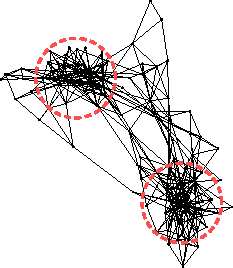
\includegraphics[width=\linewidth]{figs/uspol.pdf}
    \end{column}
    \end{columns}
    {\tiny\hfill 引用:『組合せ最適化から機械学習へ：劣モジュラ最適化とグラフマイニング』サイエンス社}
\end{frame}

\begin{frame}{最小カットへの帰着}
    固定された$\gamma \geq 0$に対し，
    \begin{block}{}
        \centering
    $
       \displaystyle \frac{w(E[S])}{|S|} > \gamma
    $
    を満たす$S$が存在するか？(存在するなら求めよ)
    \end{block}
    を解ければよい．（$\gamma$に関して二分探索）

    \bigskip
    つまり最小化問題
    \begin{block}{}
    \[
        \min_{S \subseteq V} \left[\gamma|S| - w(E[S]) \right] < 0
    \]
    \end{block}
    を解ければよい．

    \bigskip
    \structure{方針} この最小化問題を\alert{最小$s$--$t$カット}で表現する
\end{frame}

\begin{frame}{最小カットへの帰着}
    \begin{columns}[T]
    \begin{column}{.5\textwidth}
        \centering
    \begin{tikzpicture}[scale=1.2]
        \node[mynodes](s) at (-3, 0) {$s$};
        \node[mynodes](t) at ( 3, 0) {$t$};
        \node[mynodes](v1) at (0, 2.5) {$v$};
        \node[mynodes](v2) at (0,-2.5) {$u$};
        \node[mynodes](i) at (0,  .7) {$i$};
        \node[mynodes](j) at (0, -.7) {$j$};
        \node at ($(v1)!.5!(i)$) {$\vdots$};
        \node at ($(v2)!.5!(j)$) {$\vdots$};
        \graph[mygraph]{
            (s) ->["{\footnotesize $w(E)$}" above, sloped] {(v1), (i)} -> (t);
            (s) ->["{\footnotesize $w(E)$}" below, sloped] {(v2), (j)} -> (t);
            (i) ->[bend right, "{\footnotesize $w(ij)$}" left ] (j);
            (j) ->[bend right, "{\footnotesize $w(ij)$}" right] (i);
            (s) -- (v1);
            (v1) --["{\footnotesize $w(E)+2\gamma-d(v)$}" above, sloped] (t);
            (v2) --["{\footnotesize $w(E)+2\gamma-d(u)$}" below, sloped] (t);
        };
        \node[above=3pt of v1] {\footnotesize \bf $G$の頂点$V$};
    \end{tikzpicture}
    \end{column}
    \begin{column}{.5\textwidth}
        $d(v) := w(\delta(v))$ ... 重み付き次数
    \end{column}
    \end{columns}
\end{frame}

\againframe<1>{outline}
\end{document}
